\chapter{Experimental Boards} \hypertarget{def:eboards}{}

Boards in the experimental phase. Probably with some bugs and missing features. 

\section{Curiosity }

This is a simple PIC microcontroller development board that uses the
\hyperlink{def:PICSim}{PICSim backend simulator}.

\begin{figure}[H]
\center
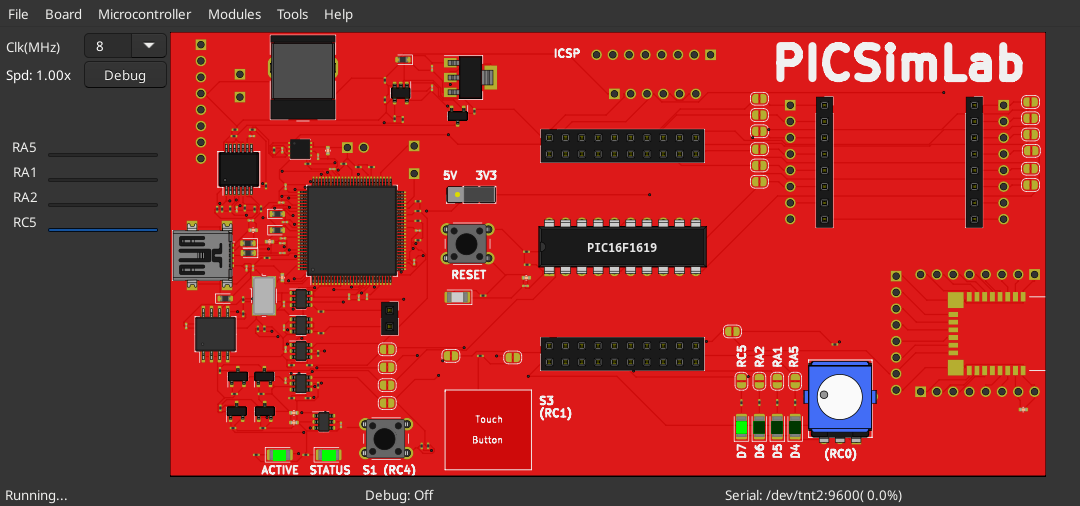
\includegraphics[width=0.7\textwidth]{img/Curiosity.png} 
\end{figure} 

\href{https://lcgamboa.github.io/picsimlab_examples/board_Curiosity.html}{Examples}

\section{Curiosity HPC}

This is a simple PIC microcontroller development board that uses the
\hyperlink{def:PICSim}{PICSim backend simulator}.

\begin{figure}[H]
\center
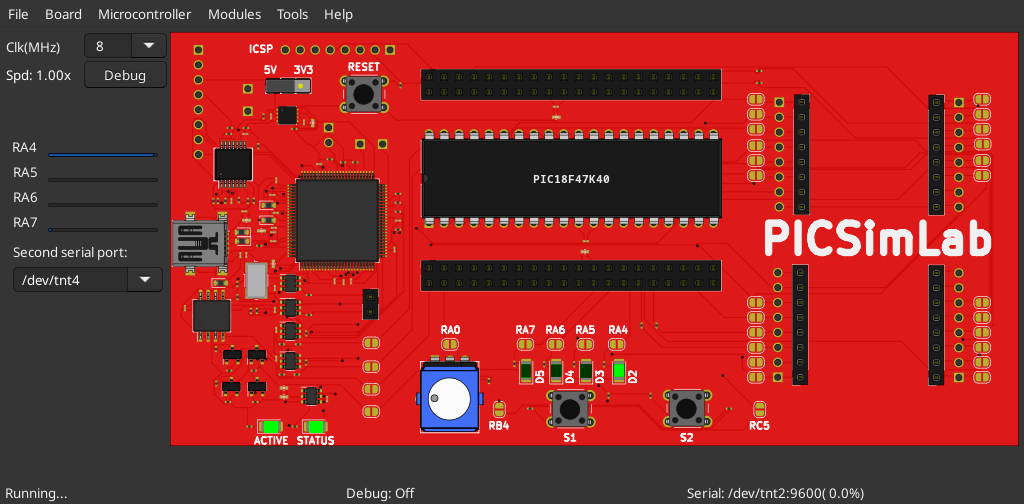
\includegraphics[width=0.7\textwidth]{img/Curiosity_HPC.png} 
\end{figure} 

\href{https://lcgamboa.github.io/picsimlab_examples/board_Curiosity_HPC.html}{Examples}

\section{Xpress}

This is a simple PIC microcontroller development board that uses the
\hyperlink{def:PICSim}{PICSim backend simulator}.

\begin{figure}[H]
\center
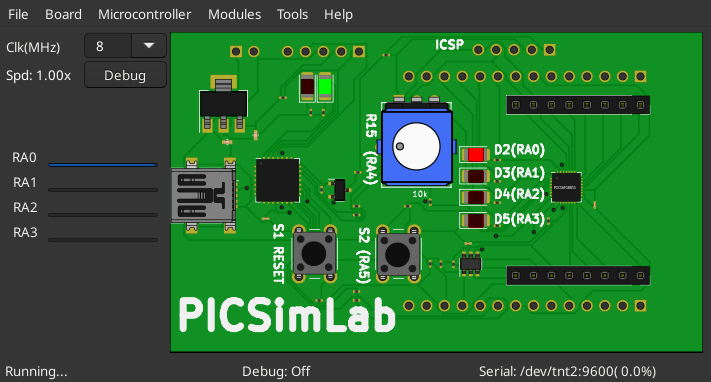
\includegraphics[width=0.7\textwidth]{img/Xpress.png} 
\end{figure} 

\href{https://lcgamboa.github.io/picsimlab_examples/board_Xpress.html}{Examples}

\section{Remote TCP}

It is a virtual board controlled through one TCP connection. 
Currently only supports the Risc-V simulator \href{https://github.com/mortbopet/Ripes}{Ripes} and 
uses the \hyperlink{def:remote}{remote backend simulator}.

\begin{figure}[H]
\center
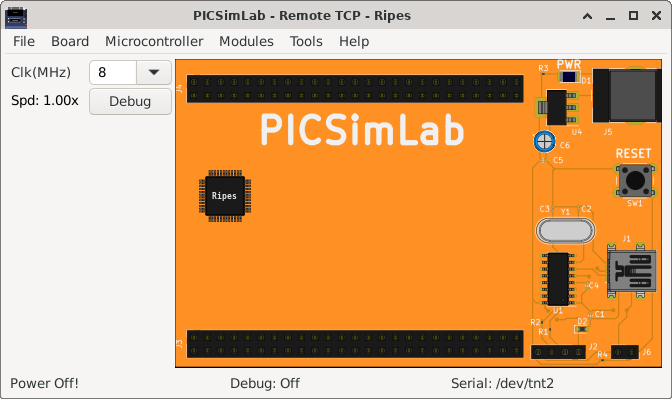
\includegraphics[width=0.7\textwidth]{img/RemoteTCP.png} 
\end{figure} 

\href{https://lcgamboa.github.io/picsimlab_examples/board_Remote_TCP.html}{Examples}


